\section{Einleitung}
Mit der zunehmenden Globalisierung steht heute praktisch jedes produzierende Unternehmen 
im internationalen Wettbewerb. Der Markt fordert hohe Flexibilität und Lieferfähigkeit, 
wobei die Kosten immer weiter sinken sollen, um wettbewerbsfähig zu bleiben.
Die japanische Firma Toyota hat diese Problematik für sich bereits in den 1950er
Jahren erkannt und eigene Lösungen dafür gesucht. So ist schliesslich im Laufe der
folgendenden Jahrzehnte das Toyota-Produktionssystem (TPS) entwickelt worden, dessen 
wesentliche Bestandteile heute auch unter den Begriffen  \emph{Just-in-Time} oder  
 \emph{Lean-Production} bekannt sind. Ein wichtiger Bestandteil des TPS ist das
Kanban-System, das vor allem von Taiichi Ohno entwickelt wurde.
\footnote{vgl. \cite{Ohno2013TPS} S.39}\\
Die vorliegende Arbeit gibt eine Einführung in die wesentlichen Methoden, 
Werkzeuge und Prinzipien des Kanban-Systems und wie mit Hilfe von Kanban eine
Just-in-Time-Produktion umgesetzt werden kann. Im zweiten Abschnitt wird hierzu
die Geschichte und Entwicklung von Kanban vorgestellt.
Im Abschnitt drei wird aufgezeigt, wie Kanban im produzierenden Betrieb 
eingeführt werden kann und wie dadurch die Wettbewerbsfähigkeit gesteigert wird. 
Eng in Verbindung mit Kanban steht der kontinuierliche Verbesserungsprozess 
(KVP), auch Kaizen genannt, was im vierten Abschnitt betrachtet wird.
Im letzten Abschnitt wird kritisch auf die Risiken einer Kanban-Einführung
eingegangen und ein Ausblick auf die zu erwartende künftige Entwicklung gegeben.\\
Für die Erstellung dieser Arbeit wurde auf relevante Fachliteratur zurückgegriffen
und teilweise auch im Internet recherchiert.


\section{Geschichte und Entwicklung von Kanban}

Das Toyota-Produktionssystem entand im Japan der Nachkriegszeit 
aus der wirtschaftlichen Notwendigkeit heraus. 
Die Produktivität eines japanischen Arbeiters betrug zu der Zeit nur einen Bruchteil der Produktivität eines Amerikaners. 
Der damalige Präsident der Toyota Motor Company Kiichiro Toyoda (1894-1952) gab daher das Ziel vor, 
die US-amerikanische Automobilindustrie innerhalb von drei Jahren  einzuholen. \footnote{vgl. \cite{Ohno2013TPS} S.36}\\
Toyotas Produktionsleiter Taiichi Ohno war der Ansicht, man müsse alle Arten von 
Verschwendung von Material und Zeit und alle unproduktiven Tätigkeiten 
beseitigen, um den Rückstand aufzuholen. Als eine Hauptursache der Ineffizienz 
und Verschwendung identifizierte man bei Toyota die Überproduktion bzw. die Produktion auf 
Halde und damit verbunden übermässige Lagerhaltung. Dadurch wird Kapital gebunden, 
die Duchlaufzeiten erhöhen sich, durch Korrosion und häufigen Transport verschlechtert
sich die Qualität der Zwischenerzeugnisse und möglicherweise müssen soger zu viel
produzierte Teile weggeworfen werden. Bedingt durch die räumliche Enge stellt die 
Lagerhaltung in Japan auch prinzipiell ein höheren Kostenfaktor dar als beispielsweise in der USA.
Künftig sollte bei Toyota die Fließproduktion \emph{Just-in-Time} erfolgen. 
Das bedeuted, dass die für die Produktion benötigten Teile zur rechten Zeit und 
nur in der benötigten Menge am Fließband ankommen.
Auf diese Weise sollte der Lagerbestand auf ein Minimum reduziert werden.
Mit den herkömmlichen Verfahren zur Produktionsplanung vom Rohstoff 
bis zum Endprodukt war das nicht zu schaffen.
Stattdessen betrachtete Ohno den Materialfluss vom Ende her, also in entgegengesetzter Richtung.
Eine Produktionsstufe entnimmt sich die benötigten Teile von der vorgelagerten Stufe oder dem Zwischenlager,
die vorgelagerte Stufe produziert darauf hin die entnommene Menge an Teilen nach.
So entsteht ein sich selbst regelndes System von Produzent und Verbraucher.
Für die Informationsübertragung in diesem Regelkreis dienen die Kanban-Karten.

Das Wort \emph{Kanban} besteht aus den zwei Zeichen {\CN 看} ( \emph{kan}=sehen)
 und {\CN 板} (\emph{ban}=Tafel, Brett) und läßt sich etwa mit Sichttafel, 
 Aushängeschild oder auch Pendelkarte übersetzen.

Im Produktionsprozess steht jede Kanban-Karte für einen Behälter einer bestimmten Größe, der eine festgelegt Anzahl von Bauteilen enthält.
Die Kanban-Karte wird an dem entsprechenden gefüllten Behälter befestigt oder eingesammelt und wieder zurück zum 
Produzenten der Teile gebracht, als Information dafür, dass wieder neue Teile benötigt werden. 
Dafür muss die Kanban-Karte verschiedene Informationen enthalten, wie Bezeichnung und Nummer der Teile, 
Anzahl der Teile pro Behälter, Art des Behälters, Produzent und Verbraucher der Teile und ggf. auch Strichcodes für die elektonische Datenerfassung.
(s. Abbildung \ref{Kanbankarte})
\begin{figure}[h]
\centering
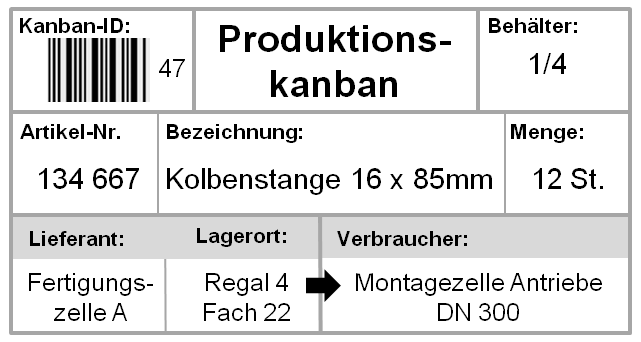
\includegraphics[width=.60\textwidth]{img/kanban-karte.png}
\caption[Beispiel einer Kanban-Karte]{Beispiel einer Kanban-Karte\footnotemark}
\label{Kanbankarte}
\end{figure}
\footnotetext{Quelle: http://www.lean-production-expert.de/lean-production/kanban-kartengestaltung.html}

Die Anzahl von Kanban-Karten für ein Bauteil oder eine Bauteilgruppe ist begrenzt, auf diese Weise soll verhindert werden, dass zu viel auf Lager produziert wird.
Der gesamte Produktionsprozess wird nun betrachtet als eine Aneinanderreihung von Quellen und Senken von Produktionsgütern, mit kleinen Zwischenlagern als Puffer.
Eine Senke nimmt sich einen Behälter aus dem Zwischenlager (Pull-Prinzip), verarbeitet alle Teile darin und füllt selbst als Quelle das nachgelagerte Zwischenlager.
Hat das nachfolgende Zwischenlager einen bestimmten Höchststand überschritten, \emph{darf nicht} weiter produziert werden.
Wird dagegen ein bestimmter Mindeststand unterschritten, so \emph{muss} wieder Nachschub produziert werden.
Auf diese Weise werden Probleme oder Engpässe schnell sichtbar und es können entsprechende Gegenmaßnahmen unternommen werden.
Andererseits können durch die mehrstufigen Zwischenlager Schwankungen bei Nachfrage, Zulieferung oder Personalstärke in gewissen Grenzen ausgeglichen werden.

Die Zwischenlager der einzelnen Produktionsstufen können auf einer \emph{Plantafel} (auch Kanban-Tafel) visualisiert werden, welche an zentraler Stelle für alle Beteiligten gut sichtbar platziert wird.
Für jede Produktionsstufe gibt es auf der Plantafel eine Spalte oder Zeile mit festen Plätzen für die Kanban-Karten.
Die Karten der leeren Behälter werden hier für jeden sichtbar plaziert, so dass auf einen Blick der Bestand der Zwischenlager erkennbar wird.


\section{Einführung von Kanban}
\subsection{Problemstellung}
Die Motivation für die Einführung der Just-in-Time-Produktion ist ist heute die gleiche wie im 20. Jahrhundert bei Toyota.
Bei gleichbleibend hoher Qualität sollen Lieferfähigkeit und Flexibilität gesteigert werden.
Ebenso sollen Durchlaufzeiten und Umlaufvermögen reduziert werden.\footnote{vgl. \cite{Geiger2011Kanban} S.12}
Hinzu kommt heute noch, dass herkömmliche PPS-Systeme einen hohen Aufwand bedeuten, 
sowohl bei der Produktionsplanung als auch bei der Erfassung von Daten zu Lagerbeständen und produzierten Gütern.
Dabei sind die eingesetzten IT-Systeme oft zu unflexibel und zu theoretisch.\footnote{vgl. \cite{Weber2014KE} S.1}\\
Trotz Einsatz moderner Technik kommt es zu Unstimmigkeiten von tatsächlichem und theoretischem Bestand, 
was eine Störung der Produktion zur Folge haben kann.
Diese nicht wertschöpfenden Tätigkeiten können durch die Einrichtung der selbstregelnden 
Steuerkreise eines Kanban-Systems eliminiert oder zumindest stark reduziert werden.\footnote{vgl. \cite{Geiger2011Kanban} S.13}\\

\subsection{Vorgehensweise}
Die Einführung der JIT-Fertigung nach dem Kanban-System sollte immer schrittweise erfolgen,
so hat man die Möglichkeit, zuerst in einem kleinen Teilbereich Erfahrung zu 
sammeln und eventuell bereite erste Verbesserungen vorzunehmen. 
Dabei fängt man gemäß dem Pull-Prinzip am Ende der Wertschöpfungskette an, 
also dem Fertigteilelager oder der Endfertigung. Schrittweise wird das Kanban-System 
dann auf die vorgelagerten Produktionstufen ausgeweitet, um zuletzt auch den Einkauf und die Lieferanten einzubeziehen.\footnote{vgl. \cite{Takeda2012SPS} S.194}
Von allen Beteiligten müssen die Kanban-Regeln verstanden sein und eingehalten werden. 
Dazu müssen sie entsprechend geschult werden und können mit Planspielen auf die Umstellungen vorbereitet werden.
Günstig ist es, die Regeln in einfacher Form für jeden sichtbar darzustellen und hier auch den 
Kanban-Beauftragten als Ansprechpartner bei Fragen und Problemen zu benennen.

\subsection{Herstellen der Kanban-Fähigkeit}
\subsubsection{Ermittlung der Kanban-Teile}
Für Kanban eignen sich grundsätzlich A-, B- und C-Teile, wobei sich bei den sehr 
werthaltigen A-Teilen die Vorteile von Kanban am ehesten zeigen. \footnote{vgl. \cite{Geiger2011Kanban} S.29}
Die infrage kommenden Teile müssen auch einer XYZ-Analyse unterzogen werden. 
Teile mit gleichmäßiger (X) oder moderat schwankender (Y) Nachfrage eignen sich gut für die JIT-Fertigung mit Kanban.
Selten produzierte Teile und Teile mit stark schwankender Nachfrage hingegen sind nicht geeignet und sollten 
weiterhin der herkömmlichen Fertigungsplanung unterliegen. Die starken Nachfrageschwankungen 
würden die vorgelagerten Regelkreise stören und damit die Produktion der anderen Teile gefährden.\footnote{vgl. \cite{Geiger2011Kanban} S.27}

\subsubsection{Verkleinerung der Losgrösse und Verkürzung der Rüstzeiten}
Um die erforderliche Flexibilität an den einzelnen Fertigungsstufen zu erreichen, 
muss von der Optimierung der Losgrößen Abstand genommen werden.\footnote{vgl. \cite{Takeda2012SPS} S.68 f.}
Andernfalls ist es nicht möglich, die benötigten Teile nur in der benötigten Menge zum geforderten Zeitpunkt herzustellen.
Der Kurvenverlauf der Gesamtkosten ist bei der 'optimalen Losgröße' relativ flach, 
so dass mit nur geringen Mehrkosten die Losgröße deutlich reduziert werden kann.\footnote{vgl. \cite{Geiger2011Kanban} S.37}
(s. Abbildung \ref{Losgroesse})
\begin{figure}[h]
\centering
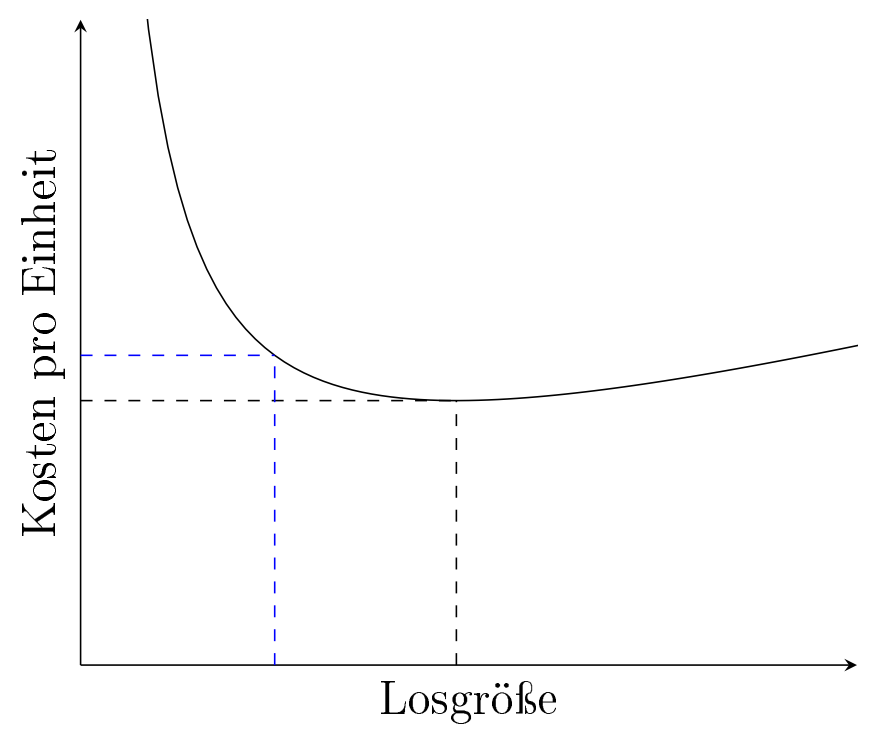
\includegraphics[width=.60\textwidth]{img/losgroessenverkleinerung.png}
\caption[Kosten bei Verkleinerung der Losgröße]{Kosten bei Verkleinerung der Losgröße\footnotemark}
\label{Losgroesse}
\end{figure}
\footnotetext{eigene Darstellung}

Letztlich muss aber auch daran gearbeitet werden, die Umrüstzeiten zu optimieren.
So ist es zum Beispiel Toyota gelungen, in seinem Hauptwerk die Zeit für Umrüstungen von 
2-3 Stunden in den 1940er Jahren auf nur 3 Minuten im Jahr 1971 zu reduzieren! \footnote{vgl. \cite{Ohno2013TPS} S.32f}

\subsection{Auswahl der Regelkreise}
\subsection{Ermittlung der Kanban-Größen}
Für die Kanban-Steuerung sind diese Kennzahlen relevant: Losgröße, Wiederbeschaffungszeit, 
Sicherheitsbestand, Maximalbestand, Kanban-Standardmenge und Kanban-Anzahl.\footnote{vgl. \cite{Geiger2011Kanban} S.36}\\

Wie bereits erwähnt sollte die \textbf{Losgröße} soweit wie möglich reduziert werden. Die positiven Effekte daraus sind  
höhere Flexibilität, geringere Lagerhaltungskosten, bessere Kundenorientierung, 
geringeres Abschreibungsrisiko, Vorteile beim Handling und Motivation der Mitarbeiter durch 
abwechslungsreichere Tätigkeit.\footnote{\cite{Geiger2011Kanban} S.36}\\

Für die \textbf{Wiederbeschaffungszeit} kann man die Erfahrungswerte mit den vorgelagerten Fertigungsstufen heranziehen.
Falls die Teile extern eingekauft werden, so muss mit dem Lieferanten eine realistische Wiederbeschaffungszeit vereinbart werden.\\

Der \textbf{Sicherheitsbestand} muss die Versorgung mit Teilen während der Wiederbeschaffungszeit ermöglichen.\\
\centerline{\textit{SBZ = DV * ( WBZ + SZ )}}
SB=Sicherheitsbestand\\
DV=Durchschnittsverbrauch pro Zeiteinheit\\
WBZ=Wiederbeschaffungszeit (in Zeiteinheiten)\\
SZ=Sicherheitszuschlag (in Zeiteinheiten)\\
Der Sicherheitszuschlag soll unvorhergesehene Bedarfsschwankungen oder Lieferprobleme
ausgleichen und sollte möglichst niedrig gewählt werden.\\

Die \textbf{Maximale Bestandsmenge} gibt an, wie viele Teile maximal im jeweiligen Kanban-Kreis vorhanden sein können.\footnote{vgl. \cite{Geiger2011Kanban} S.38}

\centerline{\textit{MB = WBZ * DV + BM + SB}}
 MB=Maximale Bestandsmenge\\
 WBZ=Wiederbeschaffungszeit (in Zeiteinheiten)\\
 DV=Durchschnittsverbrauch pro Zeiteinheit\\
 BM=Bestellmenge bzw. Losgröße\\
 SB=Sicherheitsbestand\\
Die Maximale Bestandsmenge sollte auch so weit wie möglich reduziert werden, da der Wert die Durchlaufzeit und das Umlaufvermögen beeinflußt.\\

Die \textbf{Kanban-Standardmenge} ist die Menge, die duch ein Kanban angefordert wird.
Sie sollte am besten einem vollen Behälter entsprechen und sich an der Losgröße orientieren.
Sollte die Losgröße grösser sein, z.B. weil bei einem Lieferanten immer eine bestimmte Mindestmenge angefordert werden muss, 
so werden die Kanban gesammelt, bis die Losgröße erreicht ist.\\

Die \textbf{Anzahl der Kanban} ergibt sich aus den anderen Größen:\footnote{vgl. \cite{Geiger2011Kanban} S.39}

\centerline{\textit{AK = (DV * WBZ + (1 + SF) ) / SM}}

 AK=Anzahl Kanban\\
 DV=Durchschnittsverbrauch pro Zeiteinheit\\
 WBZ=Wiederbeschaffungszeit (in Zeiteinheiten)\\
 SF = Sicherheitsfaktor\\
 SM = Standardmenge\\
Auch diese Kennzahl sollte möglichst klein gehalten werden. Sind zu viele Kanban-Karten im Umlauf so 
werden die Schwachstellen im Produktions-System durch zu hohe Lagerbestände überdeckt.
Nach Einführung des Kanban-Systems sollte im Rahmen des \textit{kontinuierlichen Verbesserungsprozess} (KVP bzw. Kaizen) 
die Anzahl der Kanban schrittweise reduziert werden. 

Glätten der Produktion, Verkleinerung der Losgrössen, Standardisierung der Teile (Takeda 2015, S. 7)\\
zuerst in einem Teilbereich, ein Team von ca 10 Personen organisiert sich eigenständig, Dauer 6-12 Monate\\
Höhe Verantwortung der einzelnen Mitarbeiter\\
Kanban-Verantwortlicher prüft und korrigiert regelmäßig die Mengen.\\

\subsection{Auswahl der Kanban-Hilfsmittel}
Produktions-Kanban, Transport-Kanban\\
Kanban-Karten\\
Kanban-Tafel\\
Behälter\\
Transportwagen\\
Stellflächen\\
-Karten, Tafel, Behälter, Stellflächen, Signallampen\\
-Gitterboxen, Europaletten, Kartonagen...\\

\subsection{Erfassung von Daten}
-Zur Kontrolle, Erstellung von Metriken, für PPS-System\\
-elektronische Systeme: Barcode, QR-Code, RFID-Etiketten (Funk)\\

\section{Kaizen: kontinuierliche Verbesserung}
- Permanentes überprüfen auf Optimierungspotential.\\
Mit grösserer Anzahl von Kanban beginnen, schrittweise reduzieren (Geiger et al 2011)\\
- Für alle sichtbare Visualisierung der Kennzahlen aus den Bereichen Mitarbeiter, Bestände, Kunden, Qualität, Sicherheit, Rüstzeiten\\
- Alle Mitarbeiter in KVP einbeziehen.\\
- Jeder kann Vorschläge machen.\\
- japanische Sichtweise: der Einzelne ist Teil des Ganzen\\
- Jeder soll Störungen und Fehler melden (bei Toyoto das gesamte Band anhalten).\\
- Dem Fehler auf den Grund gehen, 5 mal warum fragen, um das eigentliche Problem zu finden und zu beheben\\
- Fehler sollten immer zu Verbesserungen führen.\\
- Bsp: Lieferant wegen Unwetter verzögert: Sicherheitsbestand erhöhen, Dualsourcing einführen\\

\section{Risiken des Kanban-Systems}
Störung durch äußere Einflüsse, z.B. Streik, Unwetter, Vulkanausbruch, Flutkatastrophe, Unfälle.\\
-> Fokus auf Risikomanagement und Verbesserungen durch Kaizen\\

\section{Fazit und Ausblick}
Kanban ist 
